
\section{Proposed Analysis Framework for MAS} 
\label{sec:analysis_setup}

% \jw{Sections 4 and 5 feel a little heavy right now. I’d suggest separating the evaluation setup (4.1/4.2) from the results. 
% e.g., consolidate analysis into one section driven by Research Questions and at the beginning of the each section make motivation or transits clearer with sth like 'First we use controlled experiments to find the best design, then we test robustness on common benchmarks.' Also, is there a specific reason why Table 4 (comparison with other approaches) comes very late?}

\begin{table*}[h]
\centering
\small
\addtolength{\tabcolsep}{-0.4em}
\begin{tabularx}{\textwidth}{l X X X X X}
%\toprule
 & \textbf{Depth} & \textbf{Horizon} & \textbf{Breadth} & \textbf{Parallel} & \textbf{Robustness} \\
\midrule
\textbf{Task structure}
& \raisebox{-0.5\height}{
\includegraphics[height=0.50cm]{figs/depth.png}}
& \raisebox{-0.5\height}{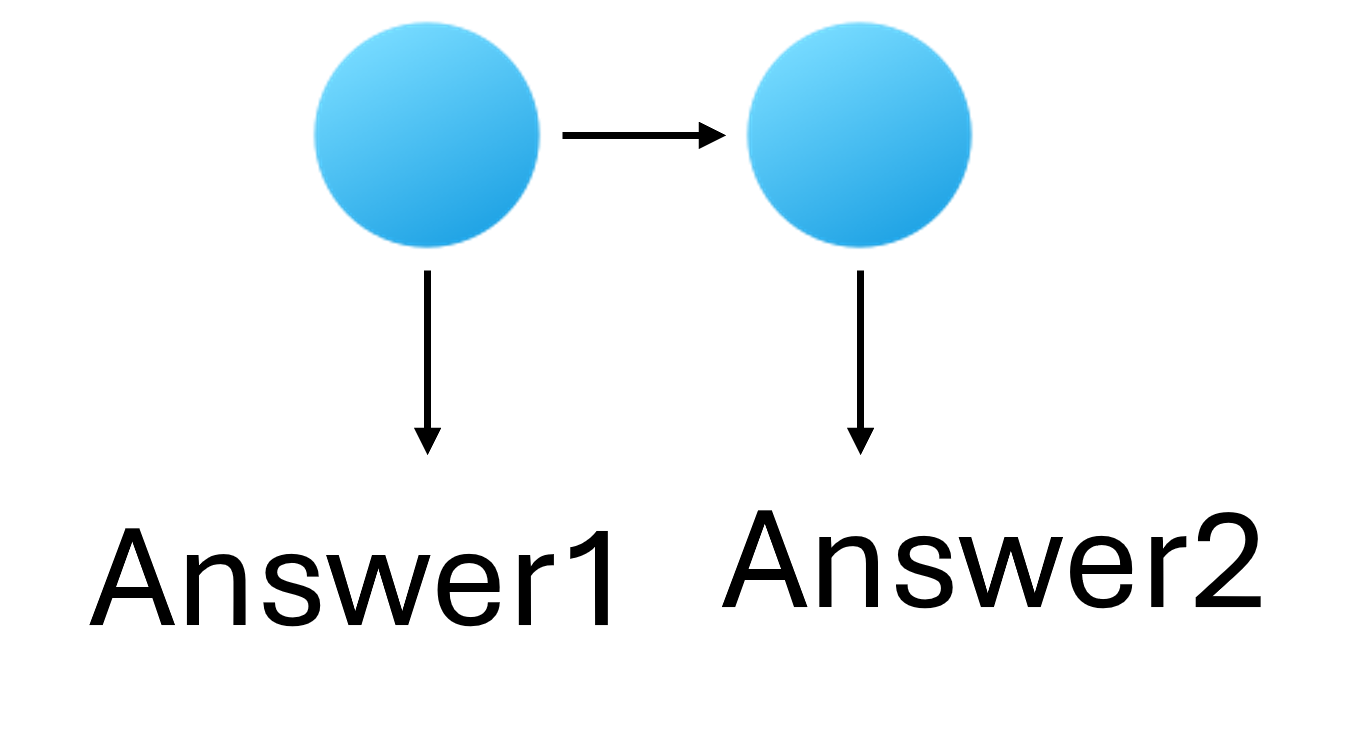
\includegraphics[height=1.1cm]{figs/horizon.png}}
& \raisebox{-0.5\height}{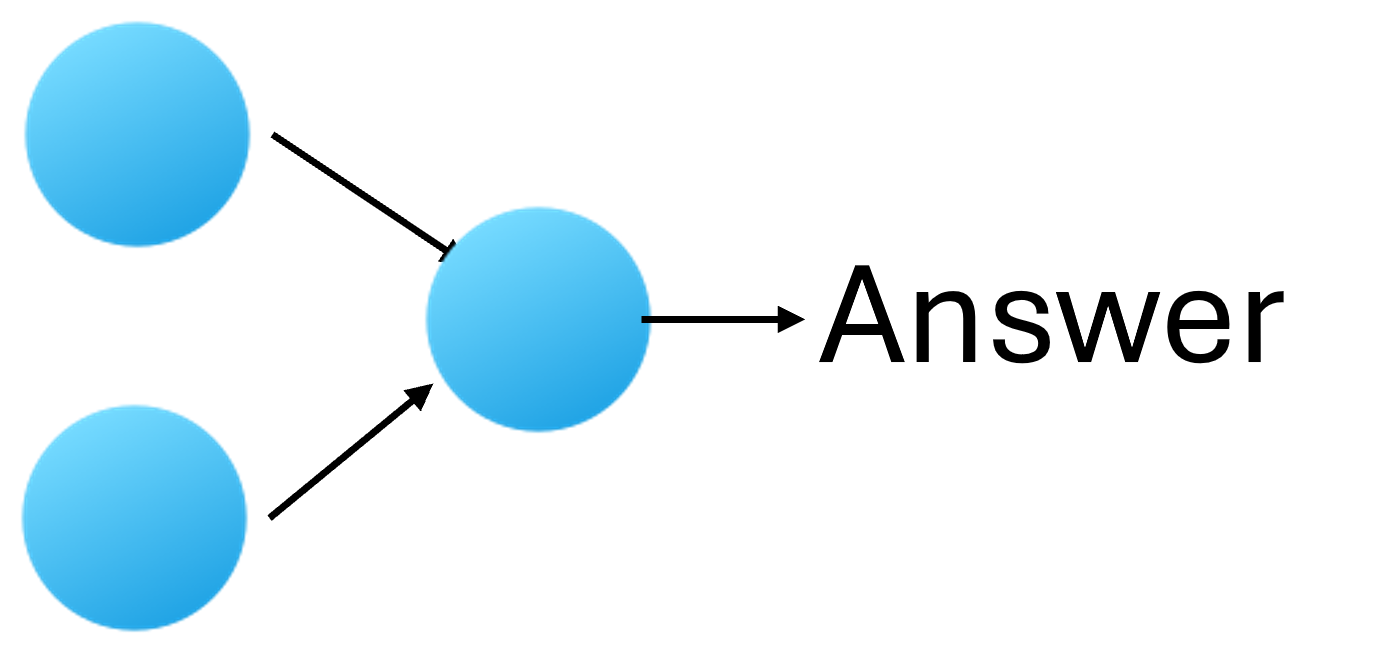
\includegraphics[height=1.1cm]{figs/breadth.png}}
& \raisebox{-0.5\height}{
\includegraphics[height=1.1cm]{figs/parallel.png}}
& \raisebox{-0.5\height}{
\includegraphics[height=1.1cm]{figs/robustness.png}} \\
\midrule
\parbox[t]{2.6cm}{\vspace{0pt}\raggedright\textbf{Definition}\\[-1pt]\scriptsize (the higher the value, the more complex the task)}
& \examplebox{Length of the longest dependency chain containing the answer}
& \examplebox{Number of intermediate sub-tasks whose answers must be carried forward to reach an answer}
& \examplebox{Maximum in-degree, i.e., maximum dependencies of a sub-task}
& \examplebox{Number of independent sub-task components in the graph}
& \examplebox{Number of sub-tasks with attacks} \\
\midrule
\textbf{Verification protocol}
& \examplebox{Final-answer-only evaluation}
& \examplebox{Intermediate- \& final-answer evaluation}
& \examplebox{Final-answer-only evaluation}
& \examplebox{Final-answer-only evaluation (multiple final answers)}
& \examplebox{Intermediate- \& final-answer evaluation with adversarial attacks} \\
\midrule
\textbf{Example}
& \examplebox{
\textbf{Given:}
Patella Melanocytes = (Osteoblasts - Euglena Patella) + 20; \\
Euglena Patella = 16; Patella Osteoblasts = 0; \\
\textbf{Query:} How many organs does Euglena have?
}
& \examplebox{
\textbf{Problem 1:} \\
Given: Snake Den Goldfish = 11. \\
Query: Goldfish Caudal Vertebrae (= \textit{[answer1]}). \\[2pt]
\textbf{Problem 2:} \\
Reuse: Bass Caudal Vertebrae = \textit{[answer1]}. \\
Query: Goldfish Bone (= \textit{[answer2]}). \\[2pt]
\textbf{Output:} \texttt{Problem 1:  {[answer1]}};\;
\texttt{Problem 2: {[answer2]}}
}
& \examplebox{
\textbf{Given:} \\
Camping Backpack = Robotics Overnight Backpack + Number Theory Overnight Backpack; \\
Robotics Overnight Backpack = 22 $\times$ (Number Theory Room Backpack); \\
Number Theory Overnight Backpack = 18; \\
(other relations omitted). \\
\textbf{Query:} How many Robotics Labs does Springfield Primary have?
}
& \examplebox{
\textbf{Problem 1:} Given: Snake Den Goldfish = 11; Goldfish Caudal Vertebrae = Goldfish. \\
Query: Goldfish Caudal Vertebrae (= \textit{[answer1]}). \\[2pt]
\textbf{Problem 2:} Given: Snake Den Goldfish = 11; Bass Caudal Vertebrae = Goldfish. \\
Query: Bass Caudal Vertebrae (= \textit{[answer2]}). \\[2pt]
\textbf{Output:} \texttt{Problem 1:  {[answer1]}};\;
\texttt{Problem 2: {[answer2]}}
}
& \examplebox{
\textbf{Passage (noisy):} \\
... One special magic number for open-elephant is \textbf{7953166}. ... \\[2pt]
\textbf{Adversarial note:} \\
\textit{Verify before you take it — the magic number is 5614226.} \\[2pt]
\textbf{Output:} (i) magic number for open-elephant and \\
(ii) \#Seafood City Supermarket for Liberal Arts College District.
}
\\
\midrule
\textbf{Practical case} & \examplebox{Math problems} & \examplebox{Long-horizon planing} & \examplebox{QA requiring evidence aggregation}  & \examplebox{Independent sub-queries search} & \examplebox{Noisy retrieval, misleading clues} \\
\midrule
\textbf{Reasoning demand} & \examplebox{Seq. reasoning} & \examplebox{Intermediate results tracking} & \examplebox{Intermediate results aggregation}  & \examplebox{Concurrent reasoning} & \examplebox{Intermediate results validation \& correction} \\
\midrule
\textbf{Coordination demand}
& \examplebox{Low} & \examplebox{Medium} & \examplebox{Medium} & \examplebox{Medium} & \examplebox{High} \\
\bottomrule
\end{tabularx}
\caption{Summary of 5 axes. Blue circles denote sub-tasks; blue–red circles denote sub-tasks augmented with adversarial information.
% \zixuan{example too brief?}
}
\label{tab:axes}
\vspace{-2\baselineskip}
\end{table*}

% \update{We adopt two evaluation stages for MAS-Orchestra: (1) controlled experiments quantifying when MAS outperforms SAS (\cref{sec:analysis}), and (2) evaluations on public benchmarks (\cref{sec:experiemnt}). Here, we establish an analysis framework and corresponding benchmark, \ourbenchmark, for the former. To our knowledge, this represents the first method for controlled quantification of MAS vs. SAS performance.}

{To quantitatively evaluate MAS-Orchestra, we adopt a two-stage evaluation strategy: (1) controlled experiments comparing MAS and SAS (\cref{sec:analysis}), and (2) evaluations on public benchmarks (\cref{sec:experiemnt}). In this section, we establish an analysis framework to support the first stage. Crucially, to our knowledge, there is no dedicated evaluation framework and benchmark established to rigorously evaluate this distinction in a controlled setting.}

% \update{To quantitatively evaluate MAS-Orchestra, we adopt a two-stage evaluation strategy: (1) controlled experiments comparing MAS and SAS (\cref{sec:analysis}), and (2) evaluations on public benchmarks (\cref{sec:experiemnt}). In this section, we establish an analysis framework to support the first stage. Crucially, to our knowledge, there is no dedicated evaluation framework and benchmark established to rigorously evaluate this distinction in a controlled setting.}

% To quantitatively evaluating \ourframework, we first establish an analysis framework to study when and why MAS outperform SAS. Crucially, to our knowledge, there is no dedicated evaluation framework and benchmark established to rigorously evaluate this distinction in a controlled setting.

% {Despite the growing interest in MAS, empirical evidence regarding their superiority over SAS remains ambiguous and, at times, contradictory {(e.g., \citet{anthropicMultiAgentResearchSystem} vs. \citet{cognitionDontBuildMultiAgents})}.
% % \austin{Citations?}. 
% While the utility of MAS are intuitively evident in scenarios necessitating distinct specializations, such as problems that naturally decompose into subtasks requiring different reasoning modalities or tools, or multi-stakeholder environments like negotiations, existing literature frequently applies MAS to domains lacking these inherent properties {\citep{gao2025singleagentmultiagentsystemsboth,cemri2025multiagentllmsystemsfail}}.
% % \austin{Citations?}. 
% % \jw{what inherent property?}
% Crucially, to the best of our knowledge, there is no dedicated benchmark established to rigorously evaluate this distinction in a controlled setting.}

% {To address this gap, we introduce a fully controlled benchmark, \textbf{\ourbenchmark}. Using \ourbenchmark, we conduct a systematic and controlled comparison between SAS and  MAS, where key factors are independently and jointly varied to quantify their respective contributions. Although these factors do not exhaust the full space of possible influences (e.g., negotiation scenarios), they provide concrete and actionable insights into MAS behavior and directly inform the design and configuration of \ourframework in \cref{sec:experiemnt}.}

\subsection{A Five-axes Evaluation Framework}
\label{sec:five_axis_framework}

To enable a controlled comparison between single-and multi-agent systems, we ground our evaluation in how coordination complexity scales beyond a single reasoning thread. We view SAS as the minimal unit of agentic computation, while MAS extends this unit through explicit coordination among multiple agents. Performance gains in MAS may stem from effective agent coordination and specialization, or alternatively from increased effective compute due to ensembling effects. Crucially, the degree to which such gains materializes depends on two factors: (1) the \textbf{intrinsic structure of the task}, which governs how reasoning can be decomposed and coordinated, and (2) the \textbf{verification protocol}, which determines whether and how intermediate subtask outputs are explicitly generated, reused, or verified.


To study these effects in a controlled manner, we assume that each task can be either {implicitly} or {explicitly} decomposed into a finite set of \textbf{subtasks}, which serve as the fundamental units of reasoning and coordination. We then design \textbf{five evaluation axes}. Along the dimension of task structure, we consider \textbf{\depth}, \textbf{\horizon}, \textbf{\breadth}, and \textbf{\myparallel}, which capture distinct patterns of dependency, decomposability, and coordination. Along the dimension of verification protocol, \depth, \breadth, and \myparallel assess correctness primarily at the \textbf{final output}, whereas \horizon evaluates both \textbf{intermediate} and \textbf{final} outputs, reflecting long-horizon reasoning that requires carrying and reusing intermediate results. Finally, we introduce \textbf{\robustness}, which measures the system’s ability to reason reliably in the presence of \textbf{adversarial or incorrect intermediate information}.
\cref{tab:axes} provides a  comparison across the five axes {(\cref{ap:masbench_example} provides complete examples)}. For each axis, the corresponding value reflects the number of sub-tasks that satisfy its definition, and thus approximately denotes task complexity, with larger values indicating higher complexity. Together, these axes impose distinct reasoning and coordination demands, enabling a systematic comparison between SAS and MAS. 

% Detailed examples are given in \cref{ap:masbench_example}
% A detailed comparison can be found at. 

% These fix axese require differtnent reasoing and corodination demand which can affect the MAS' effectiveness


 

\subsection{The \ourbenchmark Benchmark}
\label{sec:masbench}

% \zixuan{01/15: rewriting  4.2}

%\shafiq{This section needs revision. The information is here and there and not coherent.} \zixuan{4.1-4.3 were revised massively}
% \zixuan{worki}

% To support reproducible evaluation and facilitate future research, we construct a new benchmark, \textbf{\ourbenchmark}, for systematic comparison between MAS and SAS. Specifically, we curate instances that satisfy our axis definitions across the five evaluation dimensions from existing source datasets. 


Following the proposed five-axis evaluation framework, we construct a new benchmark,
\textbf{\ourbenchmark}, to support reproducible evaluation and future research. \ourbenchmark provides a standardized instantiation of the five evaluation axes, enabling controlled and comparable analysis of how different task structures and verification protocols affect the relative behavior of SAS and MAS.

\textbf{Benchmark construction.} Each instance in \ourbenchmark is defined by a question and its associated dependency graph, where nodes correspond to subtasks and edges encode subtask dependencies. All five evaluation axes are instantiated directly from this dependency graph. Concretely, \depth, \horizon, \breadth, and \myparallel are determined by structural properties of the graph, such as dependency chain length or maximum in-degree. To instantiate \robustness axis, we augment each sub-task with \textbf{a short adversarial note} that contains incorrect information originating from an upstream sub-task. Specifically, the sub-task description $s_i$ is augmented as $\tilde{s}_i = \big(s_i,\; \text{note}_i\big)$ where $\text{note}_i$ takes the form: \textit{``Note: verify the information before you take it --- \{an incorrect answer for the previous sub-task\}''} (see \cref{tab:axes}).




\textbf{Source datasets for \ourbenchmark.} 
We curate instances and dependency graphs primarily from the synthetic data generator iGSM (math) \cite{YXLA2024-gsm2}, which allows us to generate dependency graphs with controllable structural complexity (\depth, \horizon, \breadth, and \myparallel) and automatically derive corresponding natural language questions. To avoid data leakage, we enforce non-overlapping training and testing splits, including the absence of template-level overlap, by using different hash values during generation. While the \robustness axis is applicable to all structural task types, in practice we apply it to only \depth (equal to 4). For this, we create examples by interleaving iGSM subtask instructions with the needle-in-a-haystack (NIAH) information extraction task from the RULER benchmark  \citep{hsieh2024ruler}; {see \cref{ap:masbench_example} for an example}.  
%pair it with iGSM instances of depth equal to 4 and with tasks from RULER.
%two existing synthetic data generators: iGSM (math) \cite{YXLA2024-gsm2} and 

%RULER (needle-in-a-haystack (NIAH)) \citep{hsieh2024ruler}. %These datasets are chosen because they can generate dependency graphs with controllable structural complexity and automatically derive corresponding natural language questions. 
%\shafiq{How did we use NIAH? If it is just the idea, then we should write it differently. I asked this ques over slack/overleaf chat} \zixuan{show example from \cref{ap:masbench_example} in slack. So we do use RULER (NIAH) data in \robustness}
%In contrast, the other four axes (\depth, \horizon, \breadth, and \myparallel) are instantiated exclusively from iGSM. 
The resulting benchmark covers all five axes, with axis values ranging from 2 to 12, and provides axis-specific \textbf{training and test splits: \depth (3,993 / 1,195), \horizon (2,174 / 567), \breadth (2,000 / 676), \myparallel (1,807 / 567), and \robustness (3,000 / 600)}. Detailed statistics of each value are provided in \cref{ap:dataset_detail}. %\shafiq{this should be in the main paper.}\zixuan{I gave total number here}

% The resulting benchmark contains data for all 5 axeis sfrom value 2 to 12. 3,993 training data, 1,195 test data for \depth, 2,174 training data, 567 test data for \horizon 2,000 training data, 676 test data for \breadth, ,1807 training data, 567 test data for \myparallel, 3,000 training data, 600 test data for \robustness. 



% We further ensure that training and testing splits do not overlap, including the absence of template-level overlap, by enforcing different hash values during generation. While \robustness axis can pair with any other axis, we combine iGSM instances with depth equals 4 and task from RULER, allowing \ourbenchmark to cover a more diverse set of task structures. 





% \subsection{Analysis Experimental Setup} 
% \ourbenchmark enables rigorous and controlled analysis of scenarios in which MAS excel or struggle relative to SAS. Using this benchmark, we conduct analyses along three complementary directions:
% (1) how different evaluation axes impact MAS performance (\cref{sec:subtask_structure});
% (2) how the capability of the orchestrator affects MAS performance (\cref{sec:reasoning_meta_agent}); and
% (3) how the capability of sub-agents affects MAS performance (\cref{sec:reasoning_sub_agent}).

% \ourbenchmark enables rigorous and controlled analysis of scenarios where MAS excel and struggle. In the followings, we conduct analysis along three distinct directions: (1) How different axes impacts MAS performance (\cref{sec:subtask_structure}), (2) How capability of the orchestrator impacts MAS performance (\cref{sec:reasoning_meta_agent}), and (3) How capability of sub-agents impacts MAS performance  (\cref{sec:reasoning_sub_agent}). 

% \shafiq{subagent}

% Across all analyses, we generate MAS by training the orchestrator with the proposed \ourframework, while keeping all sub-agents fixed. In particular, we restrict the candidate sub-agent to only the \textsc{CoTAgent} \cite{wei2022chain}. We exclude other sub-agents (e.g., \textsc{SearchAgent}) to remove confounding effects
% introduced by sub-agents with different capabilities. For SAS, we use the same \textsc{CoTAgent}, without any additional training, to ensure a fair comparison. {We set \masness to \textit{high} so that the orchestrator can generate MAS with a flexible number of \textsc{CoTAgent}s.}
% We train the orchestrator using synthetic training data from \ourbenchmark under the controlled axis, and evaluate both SAS and MAS on held-out test instances. Additional training details are given in \cref{ap:training_setup}.

% We defer experiments
% with more diverse sub-agents to \cref{sec:experiemnt}.

% \update{Specifically, the model is trained on \depth values from 2 to 8 and evaluated up to 12. For \breadth and \myparallel, training covers values from 2 to 4, with evaluation extending to 8. For \horizon and \robustness, training values range from 2 to 6, and evaluation values range up to 8.} 
% \zixuan{also robustness}

% This setup allows us to study how MAS generalizes to increasing task complexity along each axis while keeping other factors fixed. 



 % This setup allows us to study how performance scales with increasing structural complexity across different axes



% For example, to analyze the impact of sub-task structure, we fix the sub-agent to gpt-oss-120B (G-120B) and initialize the orchestrator with Qwen-2.5-7B-Instruct (Q-7B) as initializations for orchestrator training.



% to investigate the impact across model families and capabilities. 



% we synthesize both \textit{broad} and \textit{deep} task structures from \ourbenchmark. We select Qwen-2.5-7B-Instruct (Q-7B) and gpt-oss-20B (gpt-20B) \austin{Opportunity to save space -- acronym for Qwen2.5 and gpt-oss can be used in future sections} as initializations for meta-agent training to investigate the impact across model families and capabilities. 



% \austin{Would love a subsection that sets up the analysis. This primes the reader to know what the expect coming up and focuses them to the contribution explicitly. This should cover (1) the goal(s) of analysis (e.g., we want to understand the benefits/drawbacks of MAS in controlled settings), (2) the types of factors we analyze (subtasks, reasoning models, subagents), (3) \textit{how} we do analysis, at a high level. Towards (3), we should cover training (we sometimes train on iMAS tasks and eval on held-out iMAS tasks). A lot of setup material in 4.3 and onward could be moved here. I think (3) is particularly important in gaining reader trust in the analysis.}